\section{The process architecture}
\label{sec:system}

\begin{figure*}[t]
  \centering
  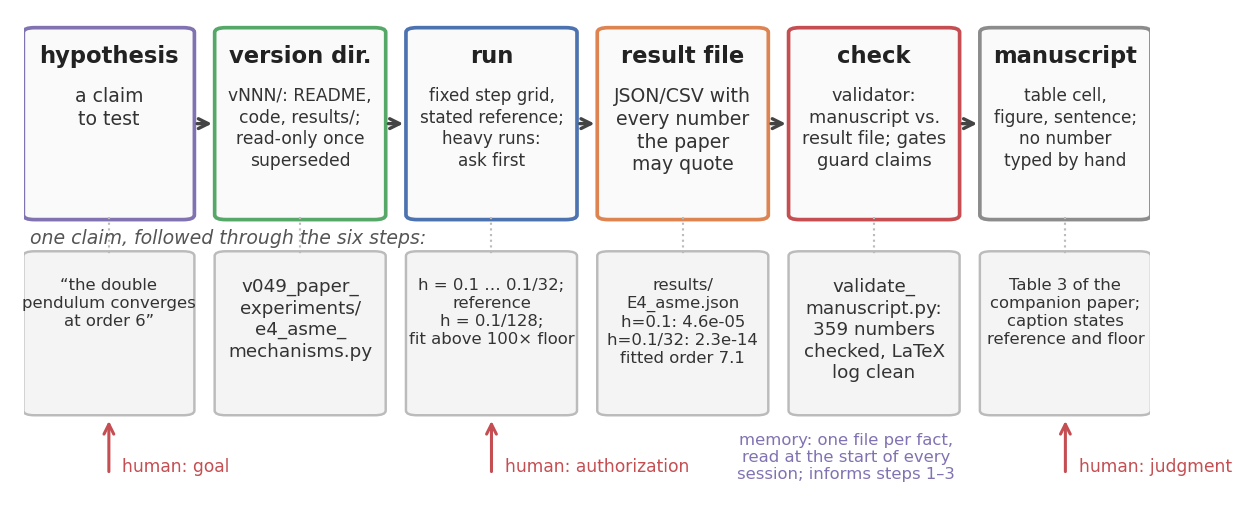
\includegraphics[width=\textwidth]{figures/fig_process.png}
  \caption{The process, and one claim followed through it. Top row: the six steps every claim
  passes through. Bottom row: the claim ``the double pendulum converges at order 6'' as it
  actually travelled: a script in a versioned directory, a run with a stated reference solution
  and a stated floor below which no order is fitted, a result file holding the numbers, a
  validator that checks each printed number against that file, and the table cell in the companion
  paper. The human enters at three points; memory carries facts between sessions; the external
  campaign runs only on explicit authorization.}
  \label{fig:process}
\end{figure*}

The agent was a general-purpose coding agent \citep{anthropic2025claudecode} with file, shell,
LaTeX, Lean and git access, working in a repository on the researcher's machine. Nothing in the
agent was specialized to the domain. What was specialized is the set of artefacts the agent had to
produce and consult, which Figure~\ref{fig:process} lays out as the path a single claim takes. We
describe the six components and, for each, the failure it was introduced to prevent.

\paragraph{Versioned exploration tree}
Every hypothesis about the method got its own directory \texttt{vNNN\_<name>} with a README, the
scripts and a \texttt{results/} folder; once superseded it became read-only and new work started a
new version. Forty-nine exist (Figure~\ref{fig:tree}a). The rule prevents the most common way an
agent loses information: editing a working script in place until the earlier state, and the reason
it was abandoned, are gone. It also makes negative results first-class: the Lobatto node swap
(v024), the projection repair (v025), matrix-free Newton--Krylov (v032) and Jacobian lagging
(v033) are preserved with the numbers that ruled them out (Figure~\ref{fig:tree}b), and the
manuscript cites them as things that were tried.

\paragraph{Evidence ledger: builders, validators, gates}
The ledger separates producing evidence from checking it. \emph{Builders} (146 scripts) read
result files and write JSON and Markdown records: convergence tables, constraint norms, Newton
statistics, claim inventories. \emph{Validators} (183 scripts) read those records and the
manuscript and assert relations between them: a quoted order equals the recorded fit, a forbidden
phrase is absent, a cited file exists with the recorded hash, a gate's preconditions hold. The
top-level validator ran $4\,896$ checks and the paper-package validator $162\,327$. \emph{Gates}
are named preconditions for stronger claims (the exact-identity gate, for instance, requires the
Lean copy in the repository to be byte-identical to the development and its axiom audit clean).
The failure this prevents is claim drift: a diagnostic row becoming a result, a consistency check becoming a proof, a number in
the text outliving the run that produced it. The ledger has a cost: by September it pinned
hundreds of phrases of a 13\,000-line manuscript and had shaped it into an audit report. When the
manuscript was rewritten (Section~\ref{sec:trajectory}) the ledger was \emph{frozen}, pointed at a
snapshot of the old paper as the historical record, and replaced for the new paper by the one
validator of the last step below.

\paragraph{Proof sandbox}
The analysis lives in a Lean~4/Mathlib project outside the working tree, with a copy in the
repository that a gate keeps synchronized. Fifty-seven theorems cover the row identities of the
implemented residual (transcribed into Lean), the perturbation lemmas with explicit constants, the
quadrature bound, the order conditions of the Gauss tableau and the local-to-global transfer. A
check script builds the project and runs an exhaustive axiom audit; two classical theorems enter as
cited results, and this is stated. The sandbox changed the paper: formalizing the theorem's
hypotheses showed that two of them follow from smoothness, and those derivations became lemmas.

\paragraph{Persistent memory}
The agent's context is finite and sessions end. A memory directory holds one file per fact, with a
one-line description and a type, and an index loaded at the start of every session. Eleven such
files exist; they record, for example, that the benchmark leaves its regular branch at
$t\approx0.6$ and all chain experiments therefore stop at $T=0.5$ (Figure~\ref{fig:incidents}b),
and that the human judged the earlier manuscript poor. The failure this prevents is repetition: an
agent that has learned why an experiment fails would otherwise run it again next session.

\paragraph{Command and authorization boundaries}
Some commands are expensive or change the meaning of the evidence. The pipeline contract lists
them: the full campaign of the method implementation is never run as a routine check, default
$h=10^{-4}$ reruns are forbidden, and the external ``source-policy'' campaign against the public
codes runs only on explicit human authorization; its driver refuses to start unless a literal
approval sentence is passed to it. The one time it ran (September~20) the human's instruction was
two words (``run B4''); the agent supplied the sentence, recorded that it had done so, and the
campaign executed 13 commands and promoted 0 of 40 rows, with the reason written down. The
boundary is procedural rather than technical, since the agent can type the sentence; what it buys
is a deliberate, recorded step.

\paragraph{Manuscript pipeline}
\label{sec:manuscript}
The rewritten manuscript is assembled from section files by a script and its figures are drawn
from result files by another, so no number is typed; a validator checks that the LaTeX log is
clean, that every number in every result table equals a value in the result file the table cites
(359 checks), that every Lean theorem named in the paper exists, and that the arXiv and flat copies
were generated from the current source. This prevents what the old ledger prevented with phrase
pins, at a fraction of the cost and without shaping the prose.
